\chapter{Gathering}
\emph{R. Kalsing, E. Markou, A. Pelc - Gathering Asynchronous Oblivious Mobile Robots In A Ring} \TODO[]{cos'e questo ?}

\paragraph{Problema del Gathering:} Convogliare un insieme di robots posizionati
tutti in un differente nodo all'interno di un grafo in un singolo nodo.\\
Nel nostro caso abbiamo studiato, all'interno dell'articolo, il problema del
Gathering in una topologia \textbf{RING} non orientata. In questo caso le
assunzioni che facciamo sono le seguenti:
\begin{itemize}
    \item Ogni robot all'inizio della computazione si trova su un nodo distinto.
    \item Ogni robot fa le proprie scelte localmente (\textbf{Autonomous}).
    \item I robot non hanno un identificatore univoco, quindi non hanno id che li
          distingue (\textbf{Anonymous}).
    \item Sono omogenei, tutti quanti eseguono lo stesso algoritmo deterministico.
    \item sono Oblivi, ovvero non hanno memoria (\textbf{Oblivious}).
    \item Sono silenti, ovvero non hanno nessun modo di comunicare esplicitamente
          tra di loro (tipo attraverso connessioni wireless) (\textbf{Silent}).
    \item Sono non-orientati, ovvero i robot non hanno modo di concludere se un
          nodo si trova a nord o a sud della loro posizione e quindi non concordano tra
          di loro su un determinato sistema di coordinate.
    \item Sono Asincroni
    \item Ogni robot si sveglia in un tempo finito e infinite volte.
    \item Multiplicity detection capability: Durante la fase di Look, che vedremo
          successivamente, i robot possono vedere un nodo che contiene più di un robot
          (chiamata, appunto, molteplicità). Esistono quattro tipi di molteplicità:
          \begin{itemize}
              \item \textbf{Global Strong}: Un robot durante la look vede tutti i
                    robot che ha la configurazione, compresi anche esattamente tutti i
                    robot in ogni determinata molteplicità su un nodo.
              \item \textbf{Global Weak}: Un robot riesce a vedere se sono presenti
                    molteplicità all'interno del ring ma non da quanti e quali robot la
                    compongono. (All'interno dell'articolo viene utilizzata questa).
              \item \textbf{Local Strong}: Un robot riesce a vedere le molteplicità
                    solamente se ne fa parte, in questo caso riesce a vedere anche quali
                    altri robot ne fanno parte insieme a lui.
              \item \textbf{Local Weak}: Un robot riesce a vedere la sua
                    molteplicità all'interno di un nodo ma non sa se all'interno del ring
                    ne sono presenti altre.
          \end{itemize}
\end{itemize}
Le assunzioni che vengono fatte sono molte poiché vogliamo capire se in questo
contesto comunque possiamo concludere qualcosa.\\

\section{Modello LOOK, COMPUTE, MOVE}
I robot si muovono solo osservando l'ambiente che li circonda, e lavorano in
cicli di Look-Compute-Move (LCM). \textbf{All'inizio i robot sono dormienti e
    sono attivati dall'avversario del problema. Trovandoci in un sistema Asincrono,
    l'avversario può svegliare i robot nell'ordine che vuole, con l'unico vincolo
    che deve svegliarli prima o poi tutti.}\\
Vediamo in dettaglio le fasi che compongono il ciclo LCM:
\begin{itemize}
    \item \textbf{Look}:\\
          Fa una foto della configurazione del sistema. In questa fase un
          determinato robot, grazie alla fotografia, riesce a vedere tutto il ring
          e la sua configurazione, ovvero quali nodi sono liberi e quelli sono
          occupati. Notare bene che la foto è instantanea, ovvero i robot che
          vengono visti sono solamente quelli sui nodi e non sugli archi (mentre
          si stanno spostando). (Dal momento in cui un robot fa la foto al momento
          in cui si muove altri robot potrebbero già aver cambiato posizione)

    \item \textbf{Compute}:\\
          In base alla configurazione percepita, il robot decide su quale nodo
          adiacente spostarsi (fa quindi un singolo step). Il robot può anche
          restare nel nodo in cui si trova.

    \item \textbf{Move}: \\
          Avviene lo spostamento
\end{itemize}
La durata di queste fasi non ha restrizioni dato che siamo in un sistema
Asincrono, basta che tutte abbiano durata finita. Da notare che i robot sono
Oblivi, quindi non si possono basare su configurazioni precedenti per effettuare
una mossa dato che non hanno memoria. Ogni mossa è basata solamente sulla Look
che effettua un robot ad ogni inizio di ciclo. Notiamo adesso alcune
considerazioni, se due robot attraversano lo stesso arco allo stesso momento non
si "incontrano", poiché la loro percezione è aggiornata solamente nella fase di
Look.\\

\section{Risultati Negativi}
\begin{theorem}
    Il gathering di 2 robot è impossibile.
\end{theorem}

\begin{proof}
    \textbf{Articolo:} Consideriamo un algoritmo di Gathering per 2 robots. In una
    qualsiasi configurazione i robot avranno la stessa vista. Consideriamo adesso
    cosa fa l'algoritmo se la distanza tra i nodi è 1. Se l'algoritmo dice ai
    robot di non muoversi allora si fallisce. Se gli dice di muoversi allora
    l'avversario effettuerà le operazioni dei due robot in maniera simultanea e
    non permetterà mai il Gathering, farà in modo quindi che i robot saranno
    sempre a distanza dispari, perchè l'avversario effettuerà sempre lo swapping
    dei due.\\
    \textbf{Mio:} Data una qualunque configurazione, ci si troverà prima o poi
    nella situazione in cui i due robot saranno su due nodi adiacenti, da qui
    l'avversario non deve far altro che far partire uno e bloccare il suo
    movimento e poi far partire l'altro. In questo caso in pratica qualunque
    decisione del protocollo si abbia i due robot o si scambieranno di posto o si
    allontaneranno.
\end{proof}

Si può concludere quindi che ci vogliono almeno 3 robot per poter risolvere il
problema.

\begin{theorem}
    Il gathering su ring è impossibile senza Multiplicity detection.
\end{theorem}

\begin{proof}
    Provo per induzione sul numero di robot (k):\\
    $k = 2 \rightarrow $ impossibile dal teorema precedente\\
    Supponiamo vero per un generico $k'< k$ e consideriamo il gathering di $k$
    robots.:\\
    Consideriamo una configurazione C subito prima che la prima molteplicità venga
    creata. In questa configurazione almeno un robot R si deve muovere su un nodo
    adiacente occupato da un altro robot per creare la molteplicità. Consideriamo
    adesso l'avversario che computa la Look e Move del robot R e solo dopo computa
    la prossima operazione di Look per i restanti robot. Il robot R creerà una
    molteplicità, riducendo quindi il numero di nodi occupati dai robot a k-1. Tutte
    le altre operazioni di Look saranno effettuate da al più $k-1$ nodi occupati dai
    robots. Dato che la multiplicity detection non è disponibile, la percezione dei
    robots sarà la stessa come nel caso $k'<k$ e quindi per ipotesi induttiva il
    gathering è impossibile.

    %Tutte le altre operazioni di Look faranno in modo che i robot vedano al più k-1
    %nodi occupati dai robot. Dato che la molteplicity detection non è disponibile,
    %la percezione dei robot sarà la stessa anche in caso di meno di k robot, ma per
    %ipotesi induttiva questo è impossibile. Avendo come obiettivo il Gathering,
    %qualunque cosa faccia l'algoritmo prima o poi dovrà far incontrare i robot, e
    %creare quindi una molteplicità. Nello specifico, la molteplicità nel nodo dove
    %finalizzare il gathering verrà prima o poi creata. Assumiamo che questa
    %molteplicità venga creata step by step, ovvero un robot alla volta; poichè
    %siamo in un sistema asincrono, anche se il nostro algoritmo volesse far
    %convogliare più robot su un solo nodo nel medesimo istante l'avversario potrà
    %sempre dilungare i tempi per fare in modo che su un nodo ci arrivi solo un
    %robot alla volta. Ci deve essere quindi un punto nel tempo in cui per la prima
    %volta questa molteplicità viene creata. Prendiamo adesso quel punto del tempo
    %in cui abbiamo almeno una molteplicità, se abbiamo una configurazione non
    %finale con una molteplicità. Se, come da ipotesi, non si avesse molteplicity
    %detection, la foto di ogni robot verrebbe percepita come se ogni nodo occupato
    %fosse occupato da un singolo robot, senza molteplicity detection queste due
    %configurazioni sarebbero indistinguibili (nel quaderno), questo significa che
    %se questi sono k+1 robot in totale, vedendola nell'altra, quelli non sono k+1
    %robot, ma sono > di k+1 robot. L'assenza di molteplicity detection quindi
    %farebbe in modo di eliminare i robot dalla vista degli altri, la percezione di
    %un robot quindi non è k+1 robot ma è "al più k robot", ma per assunzione
    %induttiva, per k robot il problema è risolvibile. Il prossimo robot che si
    %sveglia vedrà quindi solamente $k$ robot, ma per $k$ robot il teorema era vero.
\end{proof}

\begin{theorem}
    Il Gathering è impossibile se la configurazione iniziale è periodica,
    ovvero ammette più assi di simmetria (la rotazione non deve essere banale,
    ovvero non deve essere ne di 0 gradi ne di 360).
\end{theorem}

\begin{proof}
    Consideriamo una configurazione periodica che si ripete per $t>1$ volte.
    Consideriamo un avversario che ripete le stesse operazioni in ciclo, prima
    effettua la Look per tutti i robot, poi fa la Compute per tutti i robot e
    successivamente effettua la Move e così via. Da notare il fatto che i robot
    sono \textbf{oblivi}, quindi non hanno memoria delle operazioni effettuate
    precedentemente. Assumiamo configurazione periodica al giro 0, supponiamo che
    lo sia ancora al giro $r$. La vista dei i robots in tutte le $t$ copie della
    configurazione periodica sarà identica al giro $r$ e quindi la configurazione
    rimarrà periodica al round $r+1$ avendo sempre $t$ copie della configurazione.
    Per induzione la configurazione rimarrà sempre periodica non riuscendo mai a
    finalizzare il gathering. In altre parole l'avversario farà in modo di muovere
    i robot in maniera speculare in tutte le $t$ copie, non finalizzando mai il
    gathering.
\end{proof}

\begin{theorem}
    Il Gathering è impossibile se la configurazione ammette simmetria di tipo
    arco-arco.
\end{theorem}

\begin{proof}
    \ \\
    \textbf{Libro:} Consideriamo una configurazione che ammette una simmetria di tipo
    Arco-Arco. Questo significa che il numero di robot nelle due parti del ring è
    lo stesso. Consideriamo l'avversario che effettua tutte le operazioni in
    ciclo, ovvero effettua la Look per tutti i robot, poi la Compute per tutti i
    robot e poi effettua la Move per tutti i robots e così via. La configurazione
    sarà simmetrica al round 0. Supponiamo che sia simmetrica al round $r$.
    Consideriamo il robot speculare ad $R'$, ovvero dall'altra parte del ring. La
    distanza tra questi due robot è dispari. I due robot avranno la stessa vista
    al round $r$ e quindi il loro comportamento sarà lo stesso e la loro distanza
    al round $r+1$ sarà sempre dispari. Questo implica che al round $r+1$ la
    configurazione è la stessa del round $r$, quindi per induzione la
    configurazione rimane simmetrica ed il gathering è impossibile.\\

    \textbf{Mio:} È impossibile perché quando si ha questo asse le due metà del
    ring sono identiche, l'avversario potrebbe in entrambe far comportare i robot
    in maniera speculare e sincrona, non permettendo mai la creazione di una
    molteplicità. %creando mai una molteplicità.
\end{proof}

\begin{figure}[H]
    \centering
    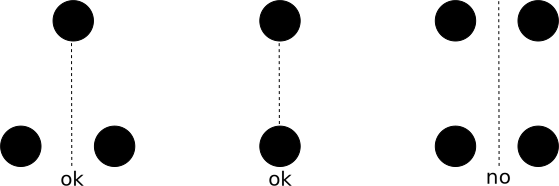
\includegraphics[scale=0.7]{images/n_48}
\end{figure}

Nelle prime due immagini effettuare il Gathering è possibile, poichè abbiamo
almeno un nodo su cui effettuarlo (quello tagliato dall'asse), nella terza
invece è impossibile, non abbiamo nodi candidati su cui effettuare gathering.

\section{Risultati Positivi}
\begin{theorem}
    Il Gathering è \textbf{risolvibile} se la configurazione iniziale è
    Asimmetrica e Aperiodica (Configurazione Rigida). In questi casi il problema del
    Gathering consiste nel riuscire a generare almeno una molteplicità.
\end{theorem}

\begin{proof}
    Assumiamo quindi che una molteplicità sia stata creata. Ai fini di far
    terminare la procedura di gathering si fa in modo che i robots che compongono
    la molteplicità non si muovano, mentre si fa in modo che tutti gli altri si
    avvicinino ad essa. Al più due a due la raggiungeranno finalizzando il
    gathering.
\end{proof}

\begin{itemize}
    \item Asimmetriche: La distanza che ha un robot dagli altri è diversa per
          tutti. Ovvero che nessun robot si può speacchiare con un altro robot
          dall'altra parte del ring.
    \item Aperiodiche: Non son presenti assi di simmetria.
\end{itemize}

La procedura, assumendo che una molteplicità sia stata creata per finalizzare il
Gathering è la seguente:

\begin{itemize}
    \item Se R è in una molteplicità allora non si muove
    \item Altrimenti:
          \begin{itemize}
              \item Se il segmento che è presente tra te (Robot) ed R NON è libero
                    allora non muoverti
              \item Altrimenti Muoviti verso la molteplicità tramite il più piccolo
                    percorso libero oppure in caso di equità in qualsiasi percorso.
          \end{itemize}
\end{itemize}

\begin{lemma}
    La procedura sopra descritta esegue il Gathering in una
    qualsiasi configurazione con una singola molteplicità.
\end{lemma}

\begin{proof}
    Questo è vero perchè un robot si muove solamente se il segmento
    tra lui e la molteplicità è libero, ed in questo caso il robot si muove
    solamente sui nodi liberi del ring. Questo implica che nessun altra molteplicità
    oltre quella esistente verrà creata. Dato che per ogni configurazione con una
    singola molteplicità è garantito che alcuni robot abbiano un segmento vuoto tra
    loro e la molteplicità, ad un certo tempo $t$ questi robot andranno verso la
    molteplicità ed al più a due a due la raggiungeranno, facendo in modo che i
    segmenti si liberino per gli altri robot, che si muoveranno di conseguenza.
\end{proof}

\section{Gathering nelle configurazioni Rigide:}
\subsection{Creazione di una singola molteplicità}
Abbiamo dedotto quindi che per finalizzare il gathering in qualsiasi
configurazione rigida, indipendentemente dal numero di robots è necessario
creare una singola molteplicità. \textbf{L'idea principale è quella di eleggere
    un singolo robot e muoverlo finchè non ne incontra un altro su un nodo,
    riuscendo quindi a creare una molteplicità e permettendo di finalizzare il
    gathering.} Fondamentale il fatto però che l'elezione di questo robot deve fare
in modo che durante il suo cammino non crei una configurazione in cui il
gathering non sia più risolvibile. Per far questo eleggiamo il robot nel
seguente modo:\\

\textbf{Elezione del robot:} Quello che distingue i robot sono le distanze che
hanno tra di loro. Da questa distanza posso ottenere due stringhe binarie
analizzando entrambi le direzioni. Devo tenere conto di entrambe le direzioni
perchè pur avendo la Asimmetria, dato che i robot non concordano sul verso, se
uno computa la stringa a sinistra, ed un altro robot computa una stringa a desta
è possibile che queste due siano uguali. Inserirò 0 se il nodo è vuoto, inserirò
1 se il nodo ha un robot sopra. (\textbf{Esempio:} 110111100). Ogni stringa
calcolata sarà chiamata Vista. \\ Poiché la configurazione è asimmetrica
necessariamente queste stringhe saranno tutte diverse, quindi è un po' come se i
robot adesso avessero degli ID. Di queste due viste, un robot sceglie quella
\textbf{minore}. Ogni robot può inoltre computare le stringhe di tutti gli altri
durante la fase di Look.\\ \'E fondamentale poter distinguere i robot perchè
così riusciamo a distinguere quello con vista minima, ovvero quella che ha il
valore più piccolo. Questo robot sarà quello che è più vicino all'intervallo di
nodi vuoti più lungo, e sarà lui il robot designato per effettuare lo
spostamento. Questo avviene nella direzione OPPOSTA all'intervallo dei nodi
vuoti e ora possono accadere due cose:
\begin{enumerate}
    \item Creiamo una molteplicità, e quindi il problema è risolto.
    \item Finiamo su un nodo vuoto, allargando quindi ulteriormente l'intervallo
          dei nodi vuoti
\end{enumerate}
Se ricadiamo sul secondo punto è necessario muovere nuovamente un altro robot,
ma siamo sicuri che si muoverà sempre quello perchè la sua vista sarà ancora la
più piccola di tutti, dato che avrà i bit ad 1 nelle posizioni \textbf{meno}
significative della vista, mentre l'altro robot che sta nella parte opposta
dell'intervallo dei nodi vuoti avrà gli 1 in posizioni più significative, e
questo determina una grandezza maggiore della vista.

%A questo punto l'idea è:\\ Si prende l'intervallo di vuoti maggiore (ce ne può
%essere più di uno) e si considerano i due robot all'estremo di questo
%intervallo. A questo punto si fa muovere il robot con stringa minima (che sarà
%accanto alla serie più lunga di nodi vuoti) verso la parte OPPOSTA a quella con
%i nodi vuoti, così da allargare questo intervallo. Dopo questo passaggio la
%sequenza di vuoti maggiori è una sola (supponendo che prima ce ne fossero state
%di più). Adesso dovrò comunque scegliere tra due robot per effettuare lo
%spostamento, ma se al passo precedente ho scelto quello con la stringa minima,
%quest'ultimo nella nuova configurazione avrà stringa ancora più piccola di
%quella di prima, quindi si muoverà sempre lui riuscendo prima o poi a creare
%una molteplicità.



A questo punto \textbf{si muove il robot con vista minima rispetto a tutti
    perchè sarà accanto alla serie più lunga di nodi vuoti, e si muove verso la
    parte opposta a quella con i nodi vuoti, allargando ulteriormente questo
    intervallo.} Questo significa che al prossimo passo il robot che sarà elettro
per lo spostamento sarà sempre lui, perchè ha comunque stringa più piccola di
tutti. Si continua così fin quando non si crea la prima molteplicità e
successivamente si applica la procedura per fare in modo che i nodi nella
molteplicità non si muovano ed i restanti si muovano verso di essa.\\

\textbf{Idea:} Prendi l'intervallo di vuoti maggiore, scegli un estremo di
questo intervallo e fai muovere il robot che ha stringa minore questo in maniera
tale da allargare ulteriormente l'intervallo degli 0. Al passo successivo la
sequenza di vuoti maggiori è una sola, dovrò scegliere eventualmente tra due
nodi e se ho fatto la scelta opportuna continuerò a far muovere lo stesso robot,
fino a quando non andrò a scontrarmi con un altro robot creando una
molteplicità.\\
\textbf{Come garantisco che si muova sempre lo stesso robot?} Se io allargo da
un estremo allora restringo dall'altro, e si muoverà quindi il robot con la
stringa massima. Poichè la configurazione è asimmetrica necessariamente queste
stringhe saranno tutte diverse, ma ci potrebbero essere stringhe uguali perchè i
robot non concordano su uno stesso verso. Quello che succede è che se uno legge
una stringa in un verso e l'altro la legge dall'altro è possibile che le due
stringhe siano uguali.\\
\textbf{Per ovviare a questo problema possiamo} fare in modo che ogni robot
computa due stringhe, sia a destra che a sinistra, delle due ne sceglie una
(quella più grande è più conveniente) e mette l'altra come suffisso (la mette
davanti) così facendo tutte le stringhe saranno diverse. Ora possiamo
effettivamente discriminare tra i vari robots. Nella fase di Look un robots può
computare anche le stringhe di tutti gli altri, quindi dopo questa fase tutti
sapranno quale sarà la stringa minima e quella massima nel Ring.\\
\textbf{Mi conviene far muovere il robot con la stringa maggiore}, che si
muoverà sul robot limitrofo e creerà la molteplicità.

\textbf{Provo da Libro:} Supponiamo che i robot M ed N a distanza Max siano
eletti per lo spostamento. Supponiamo che la distanza $a$ (la stringa) tra M ed
M' sia minore della distanza $b$ tra N ed N'. Il robot M si muoverà verso il
robot M'. Dopo questa mossa la distanza tra M ed N diventa Max + 1 e la distanza
tra M ed M' diventa $a-1$. Nessun altra distanza viene modificata. La
configurazione è ancora una volta rigida, perchè M ed N sono l'unica coppia di
vicini a distanza Max+1 e la distanza $a-1$ tra M ed M' è pioù piccola della
distanza $b$ tra N ed N'. I robot M ed N sono quindi nuovamente eletti perchè
ora c'è solo un singolo vbicino a distanza b tra N ed N' e quindi sarà ancora il
robot M che si muoverà verso M'. Ne segue che fino a quando una moltepclità non
viene creata un solo robot alla volta si muoverà sempre nella stessa
direzione.\\
In partenza la configurazione è asimmetrica, quindi di tutte le sequenze di
vuoti massimali ne posso identificare una. Una volta individuata questa, sempre
per la asimmetria posso individuare uno dei due estremi e se ho fatto la scelta
opportuna muoverò sempre lo stesso robot, che è quello con la sequenza maggiore
fin quando non creerò una molteplicità. Questo significa che se io allargo da un
estremo allora restringo e si stringe fino a quando non viene creata una
molteplicità Il protocollo da applicare potrebbe quindi essere quello di
spostare il robot con la stringa massima. Questo pur muovendosi manterrà la
stringa massima finchè non creerà una molteplicità. Da li in poi tutti gli altri
robot possono unirsi a quella.

\begin{theorem}
    Se la configurazione è aperiodica ed ammette numero dispari di robot è
    possibile effettuare gathering.
\end{theorem}

\begin{proof}
    Essendo presente un numero dispari di robot, si avrà sicuramente una simmetria
    di tipo Arco-Nodo. La procedura consiste nel far muovere questo robot in una
    qualsiasi posizione adiacente, dimostreremo che tre casi possono accadere:
    \begin{enumerate}
        \item Dopo lo spostamento si viene a creare una molteplicità. Succede quando
              il robot si sposta su un nodo dove era già presente un robot. Essendo
              presente una molteplicità allora è possibile finalizzare il gathering per il
              teorema precedente.
        \item La configurazione successiva è rigida (Asimmetrica e Aperiodica). A
              questo punto per il teorema precedente il gathering è risolvibile (il Th è
              quello delle stringhe Max).
        \item Si viene a creare un altro asse di simmetria (quello precedente è
              stato eliminato dallo spostamento del nodo sull'asse). In questo caso la
              simmetria diventa per forza di tipo Nodo-Arco. Si muove quindi il robot
              nell'asse di simmetria in un qualsiasi nodo adiacente, così facendo si
              ricadrà su uno di questi tre punti, riuscendo a finalizzare il gathering
              prima o poi. In un numero finito di passi la configurazione o diventa rigida
              oppure si crea una molteplicità [Non dimostrato].
    \end{enumerate}
\end{proof}
L'algoritmo per far questo è il seguente:
\textbf{Odd-Gathering:}
\begin{itemize}
    \item Se la configurazione è periodica allora il Gathering è impossibile
    \item Altrimenti:
          \begin{itemize}
              \item Se la configurazione possiede una singola molteplicità allora
                    applica Single-Multiplicity-Gathering.
              \item Altrimenti se la configurazione è rigida applica il Th sopra
                    difficilissimo
              \item Altrimenti muovi il robot sull'asse di simmetria in un qualsiasi
                    nodo adiacente.
          \end{itemize}
\end{itemize}

\section{Gathering in altri sistemi}
Nel precedente articolo abbiamo visto il gathering su sistemi Asincroni, ovvero
che la durata di ogni ciclo di LCM può durare in maniera diversa per ogni robot.
Può succedere quindi che un robot si svegli, effettui la Look e nello stesso
momento si sveglia un altro robot che effettua un ciclo completo di LCM prima
che il primo robot effettui la Compute. Questo poteva creare dei problemi,
poichè, nell'esatto caso sopra descritto, il primo robot effettuerà la sua Move
su una foto \textbf{obsoleta} del sistema. Vediamo quindi cosa succede con altri
sistemi:\\

\textbf{Modello Fully Synchronous (FSYNC):} Ogni ciclo di LCM ha la stessa
durata per ogni robot; la mossa avverà esattamente dopo n cicli di clock e per
tutti i robot, poichè si svegliano tutti allo stesso momento.\\
Riassumendo, in questo modello avremo:\\
|L|C|M|L|C|M|L|C|M|\\
|L|C|M|L|C|M|L|C|M|\\
|L|C|M|L|C|M|L|C|M|\\
per tutti i robot.\\

\textbf{Modello Semi Synchronous (SSYNC):} Non tutti i robot si svegliano
subito, la durata di LCM è la stessa per tutti. In questo caso avremo:\\\\
|L|C|M|L|C|M|\\
|-|-|-|L|C|M|\\
|L|C|M|-|-|-|\\

\textbf{Vediamo alcuni esempi di problemi risolvibili in questo modello e NON
    nel modello FSYNC:}\\
Prendiamo ad esempio, in questo modello, un Ring con un numero dispari di nodi e
posizioniamo esattamente due robot. Ovunque li mettiamo la configurazione sarà
simmetrica nodo-arco. Dato il modello in cui siamo (SSYNC), abbiamo la certezza
che prima o poi entrambi si sveglieranno. Nel ciclo di LCM scelgo un nodo e
tutti si muoveranno verso il nodo scelto come finalizzatore del gathering,
quindi in questi sistemi è risolvibile. Nel mondo Asincrono questo non sarebbe
possibile, poichè se ne sposterebbe solo uno alla volta, e l'avversario potrebbe
fare in modo che l'esecuzione sia speculare, non finalizzando ma il gathering.\\
Possiamo parlare di una gerarchia tra i livelli: \textbf{FSYNC $>$ SSYNC}, due
robot gatherabili nel mondo FSYNC sono gatherabili anche nel mondo SSYNC ma non
vale il viceversa (vedi esempio sopra).

\section{Ritorno al mondo Asincrono}
Il gathering nel mondo ASYNC si è dimostrato risolubile per tutte le seguenti
configurazioni:
\begin{itemize}
    \item Aperiodiche
    \item Simmetriche ma non Arco-Arco
    \item Numero di robot maggiore di 2
    \item Configurazioni non appartenenti a SP4 (Special Four).
\end{itemize}
\textbf{Cosa sono le configurazioni SP4?} Le caratteristiche di queste
configurazioni sono le seguenti:
\begin{itemize}
    \item Simmetriche di tipo nodo-arco.
    \item Sono sempre presenti quattro robot.
    \item Ring Dispari. (Viene in automatico dai due punti precedenti)
\end{itemize}{}
Nell'esempio sul quaderno, considerando i due intervalli di nodi "liberi",
ovvero dove non sono presenti robot, su cui passa l'asse di simmetria,
l'intervallo di nodi Dispari è maggiore di quelli dei nodi Pari.\\

\textbf{Gathering SP4 su 5 nodi su FSYNC:}\\
Prendiamo ad esempio la più piccola SP4 possibile, il disegno è su quaderno. Nel
mondo asincrono le mosse sono:
\begin{itemize}
    \item I robot vicini al nodo vuoto si devono muovere verso il medesimo, ma
          l'avversario non li sveglierà entrambi, ma solo 1 e lo sposta, facendo
          spostare di conseguenza l'asse di simmetria. La configurazione diventa
          periodica e non è possibile finalizzare il gathering.
    \item L'avversario crea 2 molteplicità mandando i robot uno sopra l'altro ed
          il gathering non è risolubile perchè si crea una configurazione periodica.
    \item Uguale alla precedente ma con l'altra coppia di nodi.
    \item Mossa di Swap tra i 4 nodi aventi il robot sopra, si crea sempre la
          stessa configurazione.
\end{itemize}
Come possiamo notare dai quattro punti precedenti, per ogni mossa c'è sempre una
contromossa dell'avversario che fa fallire il protocollo. Si conclude che il
gathering nelle SP4 su 5 nodi non è risolubile.\\

\textbf{Gathering SP4 su 7 nodi su FSYNC:} Non risolvibile, esempi sul quaderno
viola di carpi. \textbf{Gathering SP4 su 9 nodi su FSYNC:} Non risolvibile.
Nello specifico, c'è una determinata configurazione (posizionamento di robot sui
nodi) che crea un sacco di problemi, per provare tutte le possibili opzioni di
posizionamento ci si mette un tempo lunghissimo.\\ La difficoltà principale del
mondo FSYNC è che dato che l'avversario può spostare un nodo alla volta può
variare facilmente l'asse di simmetria non permettendo la finalizzazione del
gathering.

\section{Mondo SSYNC (Semisincrono)}
\textbf{Le SP4 su mondo semisincrono sono risolubili tranne la SP4 su 5 nodi.}
In questo mondo sono risolvibili perchè non esistono alcune configurazioni che
sono esattamente quelle che danno problemi nel mondo del FSYNC, ovvero quelle
che fanno sovrapporre le mosse di Look e Move.

\section{Robot su piano euclideo}
Il gathering è risolvibile in questi sistemi per un numero di robot maggiore di
2. Sono visti in questo caso come punti del piano.\\

\textbf{Smallest Enclosing
    Circle:} Un robot si sveglia, fa la foto della configurazione e deve computare
il cerchio più piccolo possibile che contiene tutti i punti. Questo cerchio sarà
unico, ne segue quindi che anche il suo centro sarà unico; i robot
finalizzeranno il gathering proprio nel centro. Le mosse quindi vanno effettuate
in maniera tale da non far spostare il centro del cerchio.\\

\properties{I punti fondamentali che determinano il cerchio o sono due sul diametro oppure sono 3 robot.}
In sostanza questa proprità dice di non far muovere i robot che potrebbero
spostare il centro. Supponiamo tutti i robot posizionati sul diametro
perfettamente stabili, essi avranno tutti la stessa vista e quindi la mossa la
possono fare tutti, in questa configurazioni non è possibile lasciare 3 robot o
2 sul diametro, l'unica soluzione è muoverli tutti assieme verso il centro.
Siamo però in un sistema asincorno, quindi non tutti si svegliano insieme.

